\documentclass[11pt, oneside]{article}
\usepackage[margin=1in,letterpaper]{geometry}
\usepackage{times}
\usepackage{graphicx}
\usepackage{amssymb,amsmath,mathtools}
\usepackage{array}
\usepackage{longtable}
\usepackage{color}
\usepackage[T1]{fontenc}
\usepackage{sectsty}
\usepackage[normalem]{ulem}
\usepackage{tikz}
\usetikzlibrary{decorations.pathmorphing,decorations.markings,calc,arrows.meta,intersections}
\usepackage{float}
\usepackage{pgfplots}
\pgfplotsset{compat=1.17}
\sectionfont{\fontsize{12}{12}\selectfont}
\subsectionfont{\fontsize{11}{11}\selectfont}
\subsubsectionfont{\normalsize\itshape\mdseries}

\renewcommand\labelitemi{{\boldmath$\cdot$}}
% NOTE: dots at every level; the handwritten dashes are set explicitly with \item[--].
\renewcommand\labelitemii{\labelitemi}
\renewcommand\labelitemiii{\labelitemi}
\renewcommand\labelitemiv{\labelitemi}

%%%%%%%%%%%%%%%%%%%%%%%%%%%%%%%%%%%%%
% Notation: symbols follow ../variables_master.tex. Renames that apply existing instructor decisions (each also marked
% at first use):
%   - wavenumber K -> k and Boltzmann K_B -> k_B (D14);
%   - incident field E_0, E_0h, E_0v, E_0p -> E^i, E^i_h, E^i_v, E^i_p (D27 and the handoff rule: EM amplitudes carry no
%     subscript 0);
%   - oscillator energy E and quantum of energy Delta E -> script E, Delta script E (D95, D100); the handwritten
%     accented energies (E and U with a tilde-like accent, L8) -> script E_ex (the tilde is reserved for complex
%     counterparts; flagged as D126);
%   - "principal quantum number" n (Planck oscillator) -> vibrational quantum number n_vib (L11, D99, D101).
% Relabeled because the handwritten subscript contradicts the definition: u_omega, B_omega -> u_f, B_f (per unit
% ordinary frequency f; see the NOTE at Eq. e:uf).
% Instructor decisions (2026-09-30, master table D117-D136): renamed (resolved): Stefan-Boltzmann constant sigma ->
% sigma_SB (D117); polarizability alpha -> alpha_pol (D118); scattering angle phi -> Theta, as in Liou (D119); dipole
% fields E_s, E_I, E_R -> E_stat, E_ind, E_rad (D121); scattered field (handwritten E, E_h, E_v where they denote the
% field scattered by the dipole) -> E^s, E^s_h, E^s_v, with E the total field and E^i the incident field (D136);
% total energy of the oscillators (handwritten E) -> script E_tot (D126; the single-oscillator script E and script
% E_ex stay). Kept (approved): the rest of D117-D136. Text decisions: Sun's peak written "blue"; "absorption by
% oxygen" corrected to "ozone"; the break in the Fig. 2 cavity wall is the small hole.
% Not triggered in this lecture (no optical depth, mu = cos theta, or asymmetry factor): F2, F6, F11.
% Units: the Rayleigh derivation (Sec. 1) follows Liou's Gaussian units (E = p'' sin(theta)/(c^2 R); alpha has the
% dimension of volume); see the NOTE at Eq. (e:Efar).
% Main reference checks: Liou (2002), Sec. 1.2 (pp. 9-13), Eqs. 1.2.1-1.2.11; Sec. 3.3.1 (pp. 87-94),
% Eqs. 3.3.1-3.3.22; App. A (pp. 523-524), Eqs. A.1-A.9. Ulaby & Long (2014), Sec. 6-2 (p. 229), Eqs. 6.2-6.6;
% Sec. 8-5.3 (p. 344), Eqs. 8.41-8.45.
%%%%%%%%%%%%%%%%%%%%%%%%%%%%%%%%%%%%%

\title{Ge158 Lecture 12: Atmospheric Scattering and Black Body Radiation (or Why Is the Sky Blue?)}
\author{Brent Minchew}
\date{}

\setlength{\emergencystretch}{1.5em}
\renewcommand{\topfraction}{0.85}
\renewcommand{\textfraction}{0.1}
\renewcommand{\floatpagefraction}{0.75}
\begin{document}
\maketitle

\noindent\underline{\textbf{Topics covered}}
\begin{itemize}
	\item Rayleigh scattering
	\item Mie scattering
	\item Planck's law
\end{itemize}

%%%%%%%%%%%%%%%%%%%%%%%%%%%%%%%%%%%%%
% NOTE: section heading from the handwritten underlined heading "Rayleigh Scattering" (page L1).
\section{Rayleigh scattering}
\label{s:rayleigh}

\begin{itemize}
	% NOTE: checked against Liou 2002, p. 87 (Sec. 3.3.1.1).
	\item Describes scattering from spherical particles whose radius $r \ll \lambda$ ($\lambda \equiv$ EM wavelength)\\
	$\Rightarrow$ Phase of EM wave $\approx$ constant
	% NOTE: checked against Liou 2002, p. 87 ("the simplest and in some ways the most important example of a physical
	% law of light scattering").
	\item This is simplest and very important models of EM scatter $\rightarrow$ major implications for RS
	\item Derivation
	\begin{itemize}
		% NOTE: checked against Liou 2002, p. 87.
		\item[--] Consider small, homogeneous, isotropic, spherical particle w/ $r \ll \lambda$ (assume molecule-size particle)
		% NOTE: the handwritten incident field E_0 is written E^i (master table D27 and the handoff rule: EM amplitudes
		% carry no subscript 0; superscript i = incident).
		\item[--] Define incident $\mathbf{E}$ field $\mathbf{E}^i$ and let $\mathbf{E}$ be total field ($\mathbf{E} = \mathbf{E}^i + \mathbf{E}$ field caused by electric dipole)
		\item[--] Define induced dipole moment
		% NOTE: handwritten alpha written alpha_pol (instructor decision, master table D118).
		\begin{equation}
			\label{e:p0}
			\mathbf{p}_0 = \alpha_\mathrm{pol}\mathbf{E}^i
		\end{equation}
		where
		\begin{itemize}
			% NOTE: checked against Liou 2002, Eq. 3.3.1 (p. 87): "In general, alpha is a tensor ... In the very
			% common case where these two vectors coincide, alpha is a scalar." alpha is flagged against the
			% attenuation constant (master table D118).
			\item[] $\alpha_\mathrm{pol} \equiv$ polarizability -- an intrinsic material property that is related to the dielectric constant
			\item[$\hookrightarrow$] In general, $\alpha_\mathrm{pol}$ is a 2$^\text{nd}$-order tensor but can often be assumed to be a scalar\\
			$\rightarrow$ we will take the scalar approximation
		\end{itemize}
		\item[--] As we discussed way back in Lecture~1, applied electric field causes dipole to oscillate in a plane that is normal to propagation vector because EM waves are transverse waves ($\mathbf{E}$, $\mathbf{H}$, and $\hat{\mathbf{k}}$ are mutually orthogonal)
		\item[--] Oscillating dipole emits EM radiation $\rightarrow$ ``the scattered wave''
		% NOTE: "Griffiths 2013" is presumably D. J. Griffiths, Introduction to Electrodynamics, 4th ed. (2013) (outside
		% source, not checked).
		% The subscripts s, I, R (static, induction, radiation) are kept as handwritten; R also denotes the distance
		% and I the intensity in this lecture (master table D121).
		\item[--] It can be shown (see Griffiths 2013) that dipole field at distance $R$ from dipole can be represented as sum of
		% NOTE (page L2): handwritten reads E_R ~ (1/R^3) d^2p/dt^2 for the radiation field; corrected to 1/R because
		% the radiation (far) field of an oscillating dipole falls off as 1/R (the far-field formula below, Eq.
		% e:Efar, on the same page; Liou 2002, Eq. 3.3.2, p. 88; outside source, not verified against a copy: Jackson,
		% Classical Electrodynamics, Sec. 9.2). The three terms scale as
		% 1/R^3, 1/R^2, 1/R, which is why the radiation field dominates in the far field.
		\begin{enumerate}
			% NOTE: handwritten E_s, E_I, E_R written E_stat, E_ind, E_rad (instructor decision, master table D121).
			\item[1)] Static field $\mathbf{E}_\mathrm{stat} \sim \dfrac{1}{R^3}\,\mathbf{p}$
			\item[2)] Induction field $\mathbf{E}_\mathrm{ind} \sim \dfrac{1}{R^2}\,\dfrac{d\mathbf{p}}{dt}$
			\item[3)] Radiation field $\mathbf{E}_\mathrm{rad} \sim \dfrac{1}{R}\,\dfrac{d^2\mathbf{p}}{dt^2}$
		\end{enumerate}
		% NOTE: checked against Liou 2002, Eq. 3.3.2 (p. 88), E = (1/c^2)(1/r)(d^2 p/dt^2) sin(gamma), with gamma (Liou) =
		% theta here (master table D120). This is in Gaussian units, as is the rest of the Rayleigh derivation (Liou,
		% p. 87: alpha "has the dimension of volume"); in SI, the right side carries an extra factor 1/(4 pi eps_0)
		% (outside source, not verified against a copy: Jackson, Sec. 9.2), equivalently alpha -> alpha/(4 pi eps_0) in Eqs. (e:Escat)-(e:Isize). The
		% parenthetical remark below is added.
		% NOTE: handwritten E (the field scattered by the dipole) written E^s (instructor decision, master table D136).
		\item[--] In far-field ($R \gg \lambda$), radiation dominates, and it can be shown
		\begin{equation}
			\label{e:Efar}
			\mathbf{E}^s = \frac{1}{c^2R}\,\frac{\partial^2\mathbf{p}}{\partial t^2}\sin\theta
		\end{equation}
		where $\theta \equiv$ angle between scattered dipole moment $\mathbf{p}$ and direction of observation\\
		(Gaussian units, as in Liou; in SI the right side carries a factor $1/(4\pi\varepsilon_0)$; equivalently, replace $\alpha_\mathrm{pol}$ by $\alpha_\mathrm{pol}/(4\pi\varepsilon_0)$ in what follows)
		% NOTE: checked against Liou 2002, Eq. 3.3.3 (p. 88), p = p_0 exp(-ik(r - ct)), written here with e^{j omega t}
		% (Conventions); the complex time-dependent form is written without a tilde, as in Lecture 4.
		\item[--] Scattered dipole moment can be written
		\begin{equation}
			\label{e:p}
			\mathbf{p} = \mathbf{p}_0\,e^{j(\omega t - kR)}
		\end{equation}
		% NOTE: checked by derivation (d^2 p/dt^2 = -omega^2 p, omega^2/c^2 = k^2, Eqs. e:p0, e:Efar, e:p) and against
		% Liou 2002, Eq. 3.3.4 (p. 88). Here k = omega/c (handwritten K; D14).
		% NOTE: handwritten "total E-field" and E written "scattered E-field" and E^s (instructor decision, master table
		% D136): Eq. (e:Escat) (like Eq. e:Efar) is the field scattered by the dipole (Liou 2002, p. 88: "the scattered
		% electric field"); the total field E defined above also includes E^i.
		\item[--] Thus, scattered $\mathbf{E}$-field is
		\begin{equation}
			\label{e:Escat}
			\mathbf{E}^s = -\mathbf{E}^i\,\frac{k^2\alpha_\mathrm{pol}}{R}\sin\theta\,e^{j(\omega t - kR)}
		\end{equation}
		% NOTE: checked against Liou 2002, Eqs. 3.3.5a-b (p. 88) and Fig. 3.10 (p. 89): Liou's E_r, E_l (perpendicular
		% and parallel to the plane of scattering) are the h and v components here, and gamma_1, gamma_2 are theta_1,
		% theta_2. Here h and v refer to the scattering plane (the plane containing the incident and scattered
		% directions), not to a surface (master table D133). Handwritten E_0h, E_0v written E^i_h, E^i_v (D27).
		% NOTE: handwritten E_h, E_v written E^s_h, E^s_v (scattered field; D136), and the scattering angle phi written
		% Theta, as in Liou (instructor decision, master table D119), here and below (cos^2 Theta, (1 + cos^2 Theta)/2).
		\item[--] Recall that we can represent any $\mathbf{E}$ field by orthogonal EM wave polarizations $h$ and $v$ (a.k.a., perpendicular and parallel), thus
		\begin{align}
			E^s_h &= -E^i_h\,\frac{k^2\alpha_\mathrm{pol}}{R}\,e^{j(\omega t - kR)}\sin\theta_1, \label{e:Eh}\\
			E^s_v &= -E^i_v\,\frac{k^2\alpha_\mathrm{pol}}{R}\,e^{j(\omega t - kR)}\sin\theta_2, \label{e:Ev}
		\end{align}
		where $\theta_1 = \dfrac{\pi}{2}$ by definition (see lecture notes on geometric optics)\\
		and $\theta_2 = \dfrac{\pi}{2} - \Theta$ where $\Theta \equiv$ scattering angle (angle between incident \& scattered waves)
		% NOTE: I is flagged against the free current I_f (L4) and the "intensity" terminology (master table D123,
		% D134). Checked against Liou 2002, p. 89 (I_0 = C|E_0|^2, I = C|E|^2); note that Liou's I_0 and I there are
		% intensities per solid angle (C/r^2 implies a solid angle), whereas the handwriting defines intensity as power
		% per unit area.
		\item[--] We are interested in the intensity $I$, defined as power per unit area, which is related to $\mathbf{E}$-field magnitude as
		\begin{equation}
			\label{e:IE}
			I_p \sim |E^s_p|^2
		\end{equation}
		% NOTE: handwritten reads I_p ~ |E^i_p|^2; corrected to the scattered field E^s_p because I_h, I_v, I_p are the
		% scattered intensities (Eqs. e:Ih, e:Iv below; Variables table; Liou 2002, p. 89: I = C|E|^2 for the scattered
		% field, I_0 = C|E_0|^2 for the incident field).
		% NOTE: checked against Liou 2002, Eqs. 3.3.7a-b, 3.3.8 (p. 89): sin(theta_2) = cos(phi).
		\item[--] Therefore
		\begin{align}
			I_h &= I_{0h}\,\frac{k^4\alpha_\mathrm{pol}^2}{R^2}, \label{e:Ih}\\
			I_v &= I_{0v}\,\frac{k^4\alpha_\mathrm{pol}^2}{R^2}\cos^2\Theta \label{e:Iv}\\
			\Rightarrow\quad I = I_h + I_v &= \left(I_{0h} + I_{0v}\cos^2\Theta\right)\frac{k^4\alpha_\mathrm{pol}^2}{R^2} \nonumber
		\end{align}
		% NOTE: checked against Liou 2002, Eq. 3.3.9 (p. 89), with k = 2 pi/lambda = omega/c; the handwritten box is
		% kept.
		\item[--] Let us consider case of scattering from Earth's atmosphere $\rightarrow$ sunlight is unpolarized $\Rightarrow$ $I_{0h} = I_{0v} = \dfrac{I_0}{2}$\\
		where $I_0 \equiv$ incident intensity
		\begin{equation}
			\label{e:Ray}
			\Rightarrow\quad \boxed{\begin{aligned} I &= I_0\,\frac{\alpha_\mathrm{pol}^2}{R^2}\,k^4\,\frac{1 + \cos^2\Theta}{2}\\ &= I_0\,\frac{\alpha_\mathrm{pol}^2}{R^2}\left(\frac{\omega}{c}\right)^4\frac{1 + \cos^2\Theta}{2} \end{aligned}}
		\end{equation}
		% NOTE: checked against Liou 2002, p. 87 ("discovered by Rayleigh (1871)") and p. 89.
		\item[--] This is the formula originally derived by Rayleigh in 1871
		\item[--] Take-homes
		\begin{itemize}
			\item Scattered intensity $\sim R^{-2}$ (due to spreading losses)
			% NOTE: the handwritten box encloses this bullet and its implication.
			\item[] \fbox{\parbox{0.8\linewidth}{\labelitemi\ Scattered intensity $\sim \omega^4$ (equiv.\ $\dfrac{1}{\lambda^4}$)\\
			\hspace*{1em}$\Rightarrow$ higher frequency radiation scatters more strongly}}
			% NOTE (page L5): handwritten "Lorentz-Lorentz formula" corrected to "Lorentz-Lorenz formula" (H. A. Lorentz and
			% L. Lorenz; Liou 2002, Eq. 3.3.16, p. 92: alpha = (3/(4 pi N_s)) (m^2 - 1)/(m^2 + 2), with m^2 = eps).
			% "moisture influences scattered intensity": reworded; see the NOTE below Eq. (e:LL).
			\item Scattered intensity $\sim \alpha_\mathrm{pol}^2$ $\Rightarrow$ relatable to dielectric constant $\varepsilon$ of atmosphere; can be shown that:
			\begin{equation}
				\label{e:LL}
				\alpha_\mathrm{pol} \sim \left(\frac{\varepsilon - 1}{\varepsilon + 2}\right) \qquad (\text{``Lorentz--Lorenz formula''})
			\end{equation}
			$\Rightarrow$ Intensity of scattered light increases w/ $\varepsilon$\\
			% NOTE: handwritten reads "=> moisture influences scattered intensity even in clear skies (other factors such
			% as particulates ...)"; changed to the line below because the "=>" implied that moisture raises epsilon of
			% air and so increases Rayleigh scattering, whereas moisture acts on atmospheric scattering mainly through
			% hygroscopic aerosols, whose size depends on relative humidity (Liou 2002, p. 70; p. 170: in a wet
			% environment aerosols interact with water vapor, which affects their size, shape, composition and optical
			% properties); those particles scatter in the Mie regime (Section s:mie). Neither Liou nor U&L gives the
			% optical polarizability of water vapor, so "only slightly" is the approved wording, not a sourced value
			% (instructor decision 2026-09-30).
			Moisture influences scattered intensity even in clear skies, but mainly by swelling aerosol particles (hygroscopic growth); water vapor itself changes molecular (Rayleigh) scattering only slightly (particulates will play an important role, as we will see in a bit)
			% NOTE (page L5): handwritten reads "I_v ~ cos phi"; corrected to cos^2 phi (Eq. e:Iv; Liou 2002, Eq. 3.3.7b,
			% p. 89). "horizontally polarized" here means perpendicular to the scattering plane (the h component of Eq.
			% e:Eh; master table D133). Checked against Liou 2002, p. 94, Eq. 3.3.22: at 90 degrees scattering the
			% scattered light is completely polarized (degree of polarization ~0.94 for real air, because of molecular
			% anisotropy).
			\item Polarization of light: dependence on scattering angle $\Theta$ only comes into vertically polarized term; $I_v \sim \cos^2\Theta$ $\Rightarrow$ $\Theta = \dfrac{\pi}{2}$ has only horizontally polarized light\\
			$\Rightarrow$ atmosphere acts as a polarizing filter, something that photographers who use polarizing filters will know very well
		\end{itemize}
	\end{itemize}
	% NOTE (page L6): the two bullets of page L6 are set at the top level of this section (interpretive: their
	% indentation lies between the top-level bullets of page L1 and the take-home bullets of pages L4-L5).
	% NOTE (page L6): the handwritten "Rayleigh scattering" above this line is an insertion (caret) between "the" and
	% "model". Checked: for a sphere, alpha = r^3 (n^2 - 1)/(n^2 + 2) (Gaussian units; outside source, the dielectric sphere in a uniform field, e.g., Jackson Sec. 4.4, with
	% eps = n^2; consistent with Liou Eq. 3.3.16 with 3/(4 pi N_s) = r^3 for one sphere), so alpha^2 k^4 =
	% k^4 r^6 ((n^2 - 1)/(n^2 + 2))^2 in Eq. (e:Ray). Also U&L 2014, p. 344: scattering efficiency xi_s = (8/3) chi^4 |K|^2
	% (Eq. 8.41), cross section Q_s = (2 lambda^2/(3 pi)) chi^6 |K|^2 (Eq. 8.45a), K = (n^2 - 1)/(n^2 + 2) (Eq. 8.43). r (radius) is flagged against the lag r of L7 (master table D124).
	\item An extension of the Rayleigh scattering model we just derived that accounts for particle size $r$ ($r \ll \lambda$) gives
	\begin{equation}
		\label{e:Isize}
		I = I_0\left(\frac{\omega}{c}\right)^4\frac{r^6}{R^2}\,\frac{1 + \cos^2\Theta}{2}\left(\frac{n^2 - 1}{n^2 + 2}\right)^2
	\end{equation}
	where $n^2 = \varepsilon$ ($n \equiv$ index of refraction)\\
	$\Rightarrow$ Scattered intensity scales as $I \sim r^6$ (for $r \ll \lambda$)
	\item What about when $r \gtrsim \lambda$?
\end{itemize}

%%%%%%%%%%%%%%%%%%%%%%%%%%%%%%%%%%%%%
% NOTE: section heading from the handwritten underlined heading "Mie-scattering" (page L6).
\section{Mie scattering}
\label{s:mie}

\begin{itemize}
	% NOTE: kept as handwritten. Strictly, the Rayleigh model does not ignore the internal field: it takes it as
	% uniform (quasi-static), which is what gives the factor (n^2 - 1)/(n^2 + 2); what it neglects is the variation
	% of the field (and its phase) across the particle (U&L 2014, p. 344: |n chi| << 1).
	\item Key approximation in Rayleigh scattering is that $r \ll \lambda$ meaning we can ignore the $\mathbf{E}$ field inside the particle and approximate scattered radiation as having same phase $\rightarrow$ works for clear atmosphere
	% NOTE: a crossed-out word before "phase" is not transcribed.
	\item As $r \rightarrow \lambda$, we have to allow EM phase to vary over surface and for particle to contain $\mathbf{E}$-fields $\Rightarrow$ interference
	\begin{itemize}
		\item[$\rightarrow$] generally the case when particles or aerosols are present
	\end{itemize}
	\item Formal derivation of Mie scattering beyond the scope of this course
	% NOTE (page L7): the correction series is the small-size expansion of the exact Mie solution for a nonabsorbing
	% sphere (real n) (outside sources, not verified against a copy: van de Hulst 1957; Penndorf 1962; Bohren &
	% Huffman 1983, Ch. 5). Corrections, by derivation (sympy series of the Mie coefficients a_1, b_1, a_2 in
	% x = kr) and numerics (60-digit mpmath evaluation of the exact Mie series; agreement to ~1e-8 at x = 1e-3 for
	% n = 1.33, 1.5, 2, 3):
	%   c_1: handwritten (6/5)(n^2 - 1)/(n + 2); corrected to (6/5)(n^2 - 2)/(n^2 + 2). Check: n -> 1 gives -2/5, the
	%        Rayleigh-Gans value (angle-averaged form factor of a sphere, 1 - (2/5) x^2);
	%   c_2: handwritten "-28 n^2" in the first numerator corrected to "-284 n^2"; handwritten (n^2 + 2)/(2n^2 + 2)
	%        corrected to (n^2 + 2)/(2n^2 + 3). The 1/900 term is the magnetic-dipole (b_1) and electric-quadrupole
	%        (a_2 ~ (n^2 - 1)/(2n^2 + 3)) contributions, reproduced term by term.
	%   Values: c_1 = -0.074, c_2 = -0.081 for n = 1.33; c_1 = 0.071, c_2 = -0.104 for n = 1.5.
	% c_1, c_2 are flagged against the speed of light c in the same equation (master table D135).
	% Scope (added; handwritten reads "the scattered intensity for any size spherical particle is"): reworded to "of
	% a spherical particle is, for small kr," because the series is a power series in kr, valid only for small kr,
	% not a result for any size. Also, c_1, c_2 are the coefficients of the scattered power integrated over all directions
	% (scattering efficiency relative to its Rayleigh value). At a fixed angle the intensity has an additional,
	% angle-dependent correction of order (kr)^2 (interference of the electric dipole with the magnetic-dipole and
	% quadrupole terms): python3, exact Mie amplitudes for n = 1.33, kr = 0.3: I/I_Rayleigh = 1.033 forward, 0.992 at
	% 90 degrees, 0.954 backward, vs 1 + c_1 (kr)^2 = 0.993 (angle-integrated: 0.993).
	\item It can be shown that the scattered intensity of a spherical particle is, for small $kr$,
	\begin{equation}
		\label{e:Mie}
		\boxed{I = I_0\left(\frac{\omega}{c}\right)^4\frac{r^6}{R^2}\,\frac{1 + \cos^2\Theta}{2}\left(\frac{n^2 - 1}{n^2 + 2}\right)^2\left(1 + c_1k^2r^2 + c_2k^4r^4 + \ldots\right)}
	\end{equation}
	where
	\begin{align}
		c_1 &= \frac{6}{5}\left(\frac{n^2 - 2}{n^2 + 2}\right), \label{e:c1}\\
		c_2 &= \frac{3}{175}\,\frac{n^6 + 41n^4 - 284n^2 + 284}{(n^2 + 2)^2} + \frac{1}{900}\left(\frac{n^2 + 2}{2n^2 + 3}\right)^2\left[15 + (2n^2 + 3)^2\right] \label{e:c2}
	\end{align}
	% NOTE: sentence added (scope of c_1, c_2; see the NOTE above Eq. e:Mie).
	(The coefficients $c_1$, $c_2$ are those of the scattered power integrated over all directions; at a fixed scattering angle the correction differs, e.g., for $n = 1.33$ and $kr = 0.3$ the exact ratio to the Rayleigh intensity is 1.033 forward, 0.992 at $90^\circ$, and 0.954 backward, versus $1 + c_1k^2r^2 = 0.993$.)
	\item[--] It's clear from the above that when $r \ll \lambda$ ($kr \ll 1$), the Mie scattering expression above reduces to the Rayleigh approximation.
	% NOTE: added "(Figure~\ref{f:mie})".
	\item[--] For $r \gtrsim \lambda$, interference is present causing $I$ to oscillate in frequency space. Conceptually (Figure~\ref{f:mie})
\end{itemize}

\begin{figure}[!htbp]
	\centering
	% Reproduces the handwritten sketch (page L7), element by element: vertical axis (arrowhead up) labeled I/I_0;
	% horizontal axis (arrowhead right) labeled kr; no ticks; a horizontal dashed line at the geometric optics limit,
	% with a wavy leader from the label "geometric optics limit (r >> lambda)" (left of the vertical axis) to the dashed
	% line at the axis; a thin line from the origin rising past the first peak, labeled "Rayleigh scattering (r <<
	% lambda)" with a short leader; a solid curve rising from the origin to a peak above the dashed line and then
	% oscillating about it with decreasing amplitude.
	% Curves computed (python3, exact Mie series) for a nonabsorbing sphere with n = 1.33 (water in the visible),
	% averaged over a narrow Gaussian distribution of sizes (5% standard deviation in kr) to remove the fine resonance ripple:
	% scattered power integrated over all directions, normalized by I_0 pi r^2 (the scattering efficiency, U&L 2014,
	% Sec. 8-5); geometric optics limit 2 (extinction paradox; U&L Fig. 8-19 shows the efficiencies vs chi). Rayleigh:
	% (8/3)(kr)^4((n^2 - 1)/(n^2 + 2))^2 (the scattering efficiency xi_s, U&L Eq. 8.41, p. 344), which rises much more steeply than the hand-drawn
	% straight line (the sketch is conceptual).
	\begin{tikzpicture}[>=stealth, font=\small]
		\begin{axis}[width=12cm, height=6.8cm, axis lines=left, axis line style={->},
			xmin=0, xmax=21, ymin=0, ymax=5.2, xtick=\empty, ytick=\empty,
			clip=false]
			\addplot[thick, smooth] coordinates {
				(0.05,0.000) (0.13,0.000) (0.20,0.000) (0.28,0.001) (0.35,0.002) (0.43,0.004) (0.50,0.007) (0.58,0.012) (0.66,0.020) (0.73,0.030) (0.81,0.044) (0.88,0.061)
				(0.96,0.081) (1.03,0.106) (1.11,0.134) (1.18,0.165) (1.26,0.200) (1.34,0.236) (1.41,0.275) (1.49,0.316) (1.56,0.360) (1.64,0.407) (1.71,0.460) (1.79,0.519)
				(1.87,0.585) (1.94,0.657) (2.02,0.733) (2.09,0.813) (2.17,0.893) (2.24,0.971) (2.32,1.045) (2.39,1.117) (2.47,1.187) (2.55,1.257) (2.62,1.329) (2.70,1.405)
				(2.77,1.486) (2.85,1.572) (2.92,1.661) (3.00,1.751) (3.15,1.924) (3.29,2.069) (3.42,2.205) (3.56,2.342) (3.70,2.485) (3.83,2.631) (3.97,2.769) (4.11,2.895)
				(4.24,3.011) (4.38,3.123) (4.52,3.236) (4.65,3.345) (4.79,3.443) (4.93,3.527) (5.06,3.600) (5.20,3.666) (5.34,3.730) (5.47,3.789) (5.61,3.836) (5.75,3.870)
				(5.88,3.891) (6.02,3.904) (6.16,3.912) (6.29,3.916) (6.43,3.910) (6.57,3.894) (6.70,3.867) (6.84,3.832) (6.98,3.792) (7.11,3.747) (7.25,3.697) (7.39,3.640)
				(7.52,3.576) (7.66,3.506) (7.80,3.434) (7.93,3.358) (8.07,3.281) (8.21,3.201) (8.34,3.117) (8.48,3.032) (8.61,2.946) (8.75,2.862) (8.89,2.778) (9.02,2.695)
				(9.16,2.612) (9.30,2.531) (9.43,2.452) (9.57,2.378) (9.71,2.306) (9.84,2.238) (9.98,2.174) (10.12,2.114) (10.25,2.059) (10.39,2.008) (10.53,1.963) (10.66,1.923)
				(10.80,1.888) (10.94,1.858) (11.07,1.835) (11.21,1.816) (11.35,1.802) (11.48,1.794) (11.62,1.791) (11.76,1.794) (11.89,1.802) (12.03,1.814) (12.17,1.829) (12.30,1.849)
				(12.44,1.874) (12.58,1.902) (12.71,1.933) (12.85,1.968) (12.99,2.004) (13.12,2.043) (13.26,2.083) (13.40,2.125) (13.53,2.168) (13.67,2.212) (13.81,2.256) (13.94,2.300)
				(14.08,2.344) (14.22,2.386) (14.35,2.427) (14.49,2.467) (14.63,2.506) (14.76,2.543) (14.90,2.577) (15.04,2.609) (15.17,2.637) (15.31,2.663) (15.45,2.686) (15.58,2.706)
				(15.72,2.722) (15.86,2.735) (15.99,2.745) (16.13,2.751) (16.27,2.754) (16.40,2.753) (16.54,2.749) (16.68,2.742) (16.81,2.732) (16.95,2.718) (17.09,2.702) (17.22,2.682)
				(17.36,2.660) (17.50,2.637) (17.63,2.611) (17.77,2.584) (17.91,2.554) (18.04,2.523) (18.18,2.491) (18.32,2.458) (18.45,2.425) (18.59,2.392) (18.72,2.360) (18.86,2.327)
				(19.00,2.292) (19.13,2.256) (19.27,2.222) (19.41,2.195) (19.54,2.172) (19.68,2.150) (19.82,2.121) (19.95,2.090)
			};
			\addplot[thin, domain=0:2.62, samples=80] {0.110989*x^4};
			\addplot[dashed, domain=0:20] {2};
			\node[anchor=west] at (axis cs:21.2,0) {$kr$};
			\node[anchor=east] at (axis cs:-0.3,4.5) {$\dfrac{I}{I_0}$};
			\node[align=left, anchor=north east] at (axis cs:-1.65,2.1) {geometric\\optics\\limit\\$(r \gg \lambda)$};
			\draw[decorate, decoration={snake, amplitude=1.2pt, segment length=8pt}] (axis cs:-1.6,1.95) -- (axis cs:-0.1,2.0);
			\node[anchor=west] at (axis cs:3.6,5.0) {Rayleigh scattering ($r \ll \lambda$)};
			\draw (axis cs:3.6,5.0) to[out=190, in=20] (axis cs:2.66,4.7);
		\end{axis}
	\end{tikzpicture}
	\caption{Scattered intensity (normalized by the incident intensity) versus $kr$: Rayleigh scattering for $r \ll \lambda$, oscillations due to interference for $r \gtrsim \lambda$, and the geometric optics limit for $r \gg \lambda$. Curve computed from the exact Mie solution for nonabsorbing spheres with $n = 1.33$ (averaged over a narrow range of sizes), as the scattered power integrated over all directions divided by $I_0\pi r^2$.}
	\label{f:mie}
\end{figure}
% NOTE: the caption is added.

%%%%%%%%%%%%%%%%%%%%%%%%%%%%%%%%%%%%%
% NOTE: section heading from the handwritten underlined heading "Solar radiation at the top of the atmosphere"
% (page L8).
\section{Solar radiation at the top of the atmosphere}
\label{s:solar}

\begin{itemize}
	% NOTE: checked against Liou 2002, p. 9 and U&L 2014, p. 229 ("A blackbody is defined as an idealized, perfectly
	% opaque material that absorbs all the incident radiation at all frequencies, reflecting none").
	\item Sun is well-represented as a black body (an idealized structure that absorbs all incident EM radiation regardless of frequency and incidence angle)
	% NOTE: added "(Figure~\ref{f:cavity})".
	\item Visualize black-body\\
	Large cavity w/ opaque walls and a small hole (Figure~\ref{f:cavity})
\end{itemize}

\begin{figure}[!htbp]
	\centering
	% Reproduces the handwritten sketch (page L8), element by element: an ellipse with a small break in the wall exactly
	% where the incoming ray crosses it (seen at 400 dpi; confirmed by the instructor, 2026-09-30, as the cavity's small hole); a line labeled "radiation in" entering from the upper left and reaching the lower right
	% wall (arrowhead at its end); then straight segments, each with an arrowhead at its end only: lower right -> top,
	% top -> lower left, lower left -> right, right -> left, and a short final arrow pointing right from the left wall.
	% To the right, the handwritten notes, set in the figure as in the scan.
	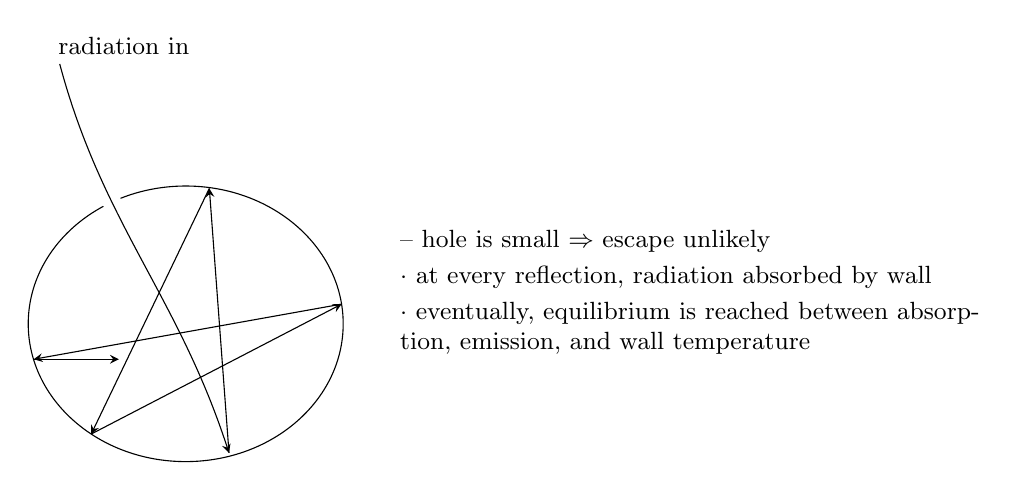
\begin{tikzpicture}[>=stealth, font=\small]
		\draw[name path=wall] (0,0) ellipse (2.0cm and 1.75cm);
		\path[name path=ray] (-1.6,3.3) to[out=-75, in=108] (0.55,-1.64);
		\path[name intersections={of=wall and ray, by={H}}];
		\fill[white] (H) circle (0.12);
		\coordinate (P1) at (0.55,-1.64);  % lower right
		\coordinate (P2) at (0.30,1.72);   % top
		\coordinate (P3) at (-1.20,-1.40); % lower left
		\coordinate (P4) at (1.98,0.25);   % right
		\coordinate (P5) at (-1.93,-0.45); % left
		\draw[->] (-1.6,3.3) node[anchor=south west, xshift=-4pt] {radiation in} to[out=-75, in=108] (P1);
		\draw[->] (P1) -- (P2);
		\draw[->] (P2) -- (P3);
		\draw[->] (P3) -- (P4);
		\draw[->] (P4) -- (P5);
		\draw[->] (P5) -- (-0.85,-0.45);
		\node[align=left, anchor=west, text width=7.4cm] at (2.6,0.4) {
			-- hole is small $\Rightarrow$ escape unlikely\\[2pt]
			$\cdot$ at every reflection, radiation absorbed by wall\\[2pt]
			$\cdot$ eventually, equilibrium is reached between absorption, emission, and wall temperature};
	\end{tikzpicture}
	\caption{A black body visualized as a large cavity with opaque walls and a small hole: radiation entering the cavity is repeatedly reflected and absorbed by the walls.}
	\label{f:cavity}
\end{figure}
% NOTE: the caption is added. Checked against Liou 2002, Fig. 1.6 and pp. 9-10.

%%%%%%%%%%%%%%%%%%%%%%%%%%%%%%%%%%%%%
% NOTE: subsection heading added (the topic "Planck's law" is listed on page L0).
\subsection{Planck's law}
\label{s:planck}

\begin{itemize}
	% NOTE: checked against Liou 2002, p. 10 (Sec. 1.2.1). "Lecture 1" refers to the damped harmonic oscillator of
	% Lecture 1.
	\item To derive theory for cavity radiation, Planck assumed atoms in wall were tiny oscillators (just like we did in Lecture~1) each w/ characteristic oscillation frequency
	\item Oscillators emit energy into and absorb energy from cavity
	\item Planck made 2 assumptions about oscillators
	\begin{enumerate}
		% NOTE (page L9): the handwritten E and Delta E are written script E and Delta script E (master table D95, D100).
		% NOTE (page L9): handwritten "n = principal quantum number"; corrected to the vibrational quantum number n_vib
		% because the principal quantum number labels the electron levels of Bohr's hydrogen atom, E_e ~ -1/n_el^2
		% (Lecture 11, Eq. e:Ee; Liou 2002, Eq. 1.3.3, p. 15), whereas hbar omega (n + 1/2) is the energy of a
		% harmonic oscillator, the vibrational energy of Lecture 11 (Eq. e:Ev; Liou Eq. 1.3.7, p. 18), which "as we saw
		% last lecture" refers to; the bare n would also clash with the index of refraction n (Secs. 1-2).
		% NOTE: kept as handwritten, but Planck's first postulate was E = n h nu~ (Liou 2002, Eq. 1.2.1, p. 10); Liou
		% adds that the correct formula for a harmonic oscillator, E = (n + 1/2) h nu~, "introduces no difference to
		% Planck's conclusions": the derivation below counts energies above the ground state (0, hbar omega,
		% 2 hbar omega, ...), and the zero-point energy hbar omega/2 does not radiate.
		\item Energy given by
		\begin{equation}
			\label{e:Eosc}
			\mathcal{E} = \hbar\omega\left(n_\mathrm{vib} + \tfrac{1}{2}\right)
		\end{equation}
		where $n_\mathrm{vib} =$ vibrational quantum number as we saw last lecture
		% NOTE: checked against Liou 2002, Eq. 1.2.2 (p. 11).
		\item Energy is quantized
		\begin{equation}
			\label{e:dE}
			\Delta\mathcal{E} = \hbar\omega
		\end{equation}
	\end{enumerate}
	% NOTE: checked against Liou 2002, p. 11.
	\item Determining emitted energy requires knowing total number of oscillators w/ freq $\omega$ for all possible states
	% NOTE (page L9): the handwritten symbols in "E > E~" and in the exponent are an E and a U, each with a tilde-like
	% accent (low-confidence reading; the two are read as the same quantity). Following Liou 2002, Eq. A.1 (p. 523;
	% "the number N in a state having energy higher by an amount epsilon"), both are written script E_ex, the energy
	% of a state above the ground state (the tilde is reserved for complex counterparts, Conventions; D95, D100);
	% master table D126. N, N_0, N_omega are flagged in D122, D125.
	% NOTE: handwritten reads "number of oscillators w/ energy E > E~"; corrected to the population of the state with
	% energy E_ex above the ground state (Liou 2002, Eq. A.1, p. 523; as in the Variables table). The number with energy
	% at or above E_ex would carry an extra factor 1/(1 - e^{-hbar omega/k_B T}).
	\item From Boltzmann statistics, number of oscillators in a state with energy $\mathcal{E}_\mathrm{ex}$ above the ground state is
	\begin{equation}
		\label{e:Boltz}
		N = N_0\,e^{-\mathcal{E}_\mathrm{ex}/k_BT}
	\end{equation}
	\begin{itemize}
		\item[] $k_B \equiv$ Boltzmann's const,
		\item[] $T \equiv$ absolute temperature.
	\end{itemize}
	\item Energy is quantized, thus $\mathcal{E}_\mathrm{ex}$ takes on discrete values
	\begin{equation*}
		\mathcal{E}_\mathrm{ex} = 0,\ \hbar\omega,\ 2\hbar\omega,\ \ldots
	\end{equation*}
	% NOTE: checked against Liou 2002, Eq. A.2 (p. 523); the sum is a geometric series, so the result is exact (Liou
	% also writes approximately-equal); "approx" kept as handwritten.
	\item Therefore, total number of oscillators w/ freq.\ $\omega$
	\begin{align}
		N_\omega &= N_0 + N_0\,e^{-\hbar\omega/k_BT} + N_0\,e^{-2\hbar\omega/k_BT} + \ldots \nonumber\\
		&\simeq \frac{N_0}{1 - e^{-\hbar\omega/k_BT}} \label{e:Nw}
	\end{align}
	% NOTE: checked against Liou 2002, Eq. A.3 (p. 523), and by derivation (sum of n x^n = x/(1 - x)^2). Handwritten
	% E (total energy of the oscillators) written script E_tot (instructor decision, master table D126), here and in
	% Eq. (e:Eavg).
	\item Total energy of oscillators comes from multiplying each term by appropriate energy level
	\begin{align}
		\mathcal{E}_\mathrm{tot} &= 0\cdot N_0 + \hbar\omega N_0\,e^{-\hbar\omega/k_BT} + 2\hbar\omega N_0\,e^{-2\hbar\omega/k_BT} + \ldots \nonumber\\
		&\simeq \frac{\hbar\omega N_0\,e^{-\hbar\omega/k_BT}}{\left(1 - e^{-\hbar\omega/k_BT}\right)^2} \label{e:Etot}
	\end{align}
	% NOTE: checked against Liou 2002, Eq. A.4 (p. 523).
	\item Average energy per oscillator is
	\begin{equation}
		\label{e:Eavg}
		\frac{\mathcal{E}_\mathrm{tot}}{N_\omega} = \frac{\hbar\omega}{e^{\hbar\omega/k_BT} - 1}
	\end{equation}
	% NOTE (page L10): handwritten u_omega; written u_f, because the quantity defined here is per unit ordinary
	% frequency f (Hz), not per unit angular frequency omega: A = 8 pi f^2/c^3 is the number of cavity modes per unit
	% volume per unit f (Liou 2002, Eqs. A.5-A.7, p. 524, u_nu~ per unit frequency nu~ in Hz; Rayleigh-Jeans u_nu~ =
	% (8 pi nu~^2/c^3) K T, Eq. A.6), and Eq. (e:Bl) converts with df/dlambda. Per unit omega the energy density would
	% be u_f/(2 pi). u_f is flagged against the lag u and u_p (master table D127); A against the areas (D128).
	\item Now define monochromatic energy density $u_f$ (energy per volume per frequency)
	\begin{equation}
		\label{e:uf}
		u_f = A\,\frac{\hbar\omega}{e^{\hbar\omega/k_BT} - 1}
	\end{equation}
	where
	\begin{equation*}
		A = \frac{8\pi f^2}{c^3} \qquad \text{with } f = \frac{\omega}{2\pi}, \qquad c \equiv \text{speed of light}
	\end{equation*}
\end{itemize}
% NOTE: checked against Liou 2002, Eq. A.6 (p. 524): for hbar omega << k_B T, u_f -> (8 pi f^2/c^3) k_B T.
The value of $A$ ensures that $u_f$ tends to the Rayleigh--Jeans law at low frequencies

\begin{itemize}
	% NOTE (page L11): handwritten "(power per unit solid angle per unit projected area => units W sr^-1 m^-2)";
	% corrected to add "per unit frequency" and Hz^-1: 2 h f^3/c^2 has units J s s^-3/(m^2 s^-2) = J m^-2 = W m^-2 Hz^-1
	% (per sr) (U&L 2014, p. 229, below Eq. 6.2: I_f "in W m^-2 sr^-1 Hz^-1"; Liou 2002, Eq. 1.2.3, p. 11:
	% "energy/area/time/sr/frequency"). W sr^-1 m^-2 are the units of the radiance integrated over the spectrum
	% (Eq. e:Ltot). The per-wavelength form B_lambda has units W sr^-1 m^-2 m^-1 = W sr^-1 m^-3.
	% NOTE (page L11): handwritten B_omega; written B_f, per unit ordinary frequency f (see the NOTE at Eq. e:uf; Liou
	% 2002, Eq. A.8, p. 524, B_nu~ = u_nu~ c/(4 pi); U&L 2014, Eq. 6.2, I_f). Per unit omega, B_omega = B_f/(2 pi).
	% B_f, B_lambda are flagged against B_1, B_2 (L6) and B^i (L5) (master table D129). Both boxes are handwritten.
	\item Finally, define spectral radiance (power per unit solid angle per unit projected area per unit frequency $\Rightarrow$ units W\,sr$^{-1}$\,m$^{-2}$\,Hz$^{-1}$)
	\begin{equation}
		\label{e:Bf}
		\boxed{B_f = \frac{u_fc}{4\pi} = \frac{2hf^3}{c^2}\left[\exp\left\{\frac{hf}{k_BT}\right\} - 1\right]^{-1}}
	\end{equation}
	% NOTE: checked by derivation (df/dlambda = -c/lambda^2) and against Liou 2002, Eq. 1.2.4 (p. 11) and U&L 2014,
	% Eqs. 6.5-6.6 (p. 229).
	which can be written in terms of wavelength as
	\begin{equation}
		\label{e:Bl}
		\boxed{B_\lambda = -B_f\,\frac{df}{d\lambda} = \frac{2hc^2}{\lambda^5}\left[\exp\left\{\frac{hc}{\lambda k_BT}\right\} - 1\right]^{-1}}
	\end{equation}
	where
	\begin{equation*}
		h = 2\pi\hbar \equiv \text{Planck's constant}
	\end{equation*}
	\item Take-homes
	\begin{itemize}
		\item[--] Strong frequency (and wavelength) dependence
		\begin{itemize}
			% NOTE (page L11): handwritten "Wein's" corrected to "Wien's" (Wilhelm Wien; Liou 2002, Sec. 1.2.3, p. 12).
			% b_W = 2.898e-3 m K kept as handwritten (python3, root of 5(1 - e^-x) = x: 2.8978e-3 m K; Liou Eq. 1.2.11,
			% p. 13: 2.897e-3). Scope added: "(of B_lambda)": Wien's law gives the peak of the per-wavelength B_lambda
			% (Liou Eq. 1.2.10); the per-frequency B_f peaks at f_max = 5.879e10 Hz/K x T, i.e., at a wavelength
			% c/f_max ~ 1.76 times longer (python3). b_W is flagged in master table D130.
			\item[$\hookrightarrow$] peak spectral radiance (of $B_\lambda$) at wavelength
			\begin{equation}
				\label{e:Wien}
				\underbrace{\lambda_\mathrm{max} = \frac{b_W}{T}}_{\text{Known as Wien's displacement}}
			\end{equation}
			where $b_W = 2.898\times10^{-3}$~m$\cdot$K $\equiv$ Wien's displacement const
			\item[$\hookrightarrow$] rapid drop off in radiance for $\lambda < \lambda_\mathrm{max}$ because it is hard for photons with energy $\gg k_BT$ (mean or characteristic energy) to be emitted
			\item[$\hookrightarrow$] long tail at $\lambda > \lambda_\mathrm{max}$ due to Boltzmann statistics
		\end{itemize}
		\item[--] Strong $T$ dependence $\rightarrow$ influences both total radiated energy and distribution
		% NOTE (page L12): handwritten "highest radiance in violet-blue spectrum"; written "blue" (instructor decision,
		% 2026-09-30): the observed top-of-atmosphere solar spectrum peaks at ~0.45-0.48 um (Liou 2002, Fig. 3.9, p. 86),
		% and a 5800 K blackbody's B_lambda peaks at 2.898e-3 m K / 5800 K = 0.50 um (Eq. e:Wien; python3); Liou,
		% pp. 93-94, puts blue light at ~0.425 um and violet at ~0.405 um, with much less energy in the violet. (Per unit
		% frequency, B_f peaks near 0.88 um.)
		\item[--] For Sun ($T \sim 5800$~K at surface), highest radiance in blue spectrum
		\begin{itemize}
			% NOTE: checked against Liou 2002, pp. 93-94 (Eq. 3.3.21, I_lambda ~ 1/lambda^4; blue light scatters about
			% 5.5 times more than red; python3: (0.650/0.425)^4 = 5.47). Liou (p. 94) explains why the sky is not violet
			% by the smaller solar energy in the violet and the eye's lower response to violet.
			% NOTE: handwritten "complemented by absorption by oxygen in atmosphere"; corrected to "ozone" (instructor
			% correction, 2026-09-30): the ozone Chappuis bands absorb weakly across the visible and near-IR, 0.44-1.18 um
			% (Liou 2002, Sec. 3.2.1.3, p. 75; see also p. 87). (Molecular oxygen has only weak red bands, A 0.762 um,
			% B 0.688 um, gamma 0.628 um; Liou Sec. 3.2.3.1, p. 82.)
			\item[$\hookrightarrow$] Recalling Rayleigh scattering intensity $\sim \omega^4$ we get blue skies (complemented by absorption by ozone in atmosphere)
			% NOTE: added (instructor decision 2026-09-30), moved from the NOTE above into the text. lambda^-4 B_lambda(5800 K)
			% peaks at lambda = hc/(x k_B T) with 9(1 - e^-x) = x, x = 8.999, i.e., 0.276 um (python3); a pure 5800 K
			% blackbody would even give ~16% more scattered light at 0.405 um than at 0.425 um (python3), so the reason is
			% the observed solar spectrum, which falls off below ~0.45 um (Liou 2002, Fig. 3.9, p. 86). Liou, p. 94: "the
			% energy contained in the violet spectrum is much less than that contained in the blue spectrum, and also
			% because the human eye has a much lower response to the violet color." Ozone (not on p. 94): the Hartley bands,
			% 0.2-0.3 um, absorb solar UV in the upper stratosphere and mesosphere (Liou p. 75), and above 0.31 um the
			% atmosphere is relatively transparent apart from scattering (p. 79); this is separate from the Chappuis-band
			% "ozone" decision above.
			\item[$\hookrightarrow$] Why not a violet sky? $\lambda^{-4}B_\lambda$ ($T = 5800$~K) keeps rising to shorter $\lambda$ (peak at $0.276~\mu$m, in the UV; ozone absorbs the solar UV below ${\sim}0.3~\mu$m), but observed sunlight holds much less energy in the violet than in the blue, and the eye is much less sensitive to violet
		\end{itemize}
	\end{itemize}
\end{itemize}

%%%%%%%%%%%%%%%%%%%%%%%%%%%%%%%%%%%%%
% NOTE: subsection heading added (page L12).
\subsection{Stefan--Boltzmann law}
\label{s:sb}

\begin{itemize}
	% NOTE (page L12): checked against Liou 2002, Eqs. 1.2.5-1.2.9 (pp. 11-12): Liou's B(T) ("total radiant
	% intensity") is L(T) here, and the "intensity" I = pi L is Liou's flux density F (W m^-2). L is a radiance
	% (W m^-2 sr^-1); in SI radiometry, "radiant intensity" is W sr^-1 (master table D134). python3: the integral is
	% pi^4/15 = 6.4939; b = 2 pi^4 k_B^4/(15 c^2 h^3) = 1.805e-8 W m^-2 sr^-1 K^-4 = sigma/pi; pi times the integral of
	% B_lambda over lambda at 5800 K equals sigma T^4 to 1e-9. L is flagged in D131, z in D132, b in D130, sigma in
	% D117 (formerly F3).
	\item Finally, in RS it is sometimes the case that we only measure the total radiant intensity
	\begin{align}
		L(T) &= \int_0^\infty B_\lambda(T)\,d\lambda \nonumber\\
		&= \frac{2k_B^4T^4}{h^3c^2}\underbrace{\int_0^\infty\frac{z^3}{e^z - 1}\,dz}_{=\,\pi^4/15} \label{e:Ltot}
	\end{align}
	where $z = \dfrac{hc}{\lambda k_BT}$
	\begin{equation*}
		\Rightarrow\quad L(T) = bT^4 \qquad \text{where } b = \frac{2\pi^4k_B^4}{15c^2h^3} = \text{const}
	\end{equation*}
	\begin{itemize}
		% NOTE: handwritten sigma written sigma_SB (instructor decision, master table D117).
		% NOTE: sigma = 5.67e-8 W m^-2 K^-4 checked (python3 from h, k_B, c: 5.6704e-8; Liou 2002, p. 12).
		\item[--] Since black body radiation is isotropic, intensity
		\begin{equation}
			\label{e:SB}
			I = \pi L = \sigma_\mathrm{SB} T^4, \qquad \sigma_\mathrm{SB} = 5.67\times10^{-8}\left[\frac{\text{W}}{\text{m}^2\text{K}^4}\right] \equiv \text{Stefan--Boltzmann const}
		\end{equation}
	\end{itemize}
\end{itemize}

%%%%%%%%%%%%%%%%%%%%%%%%%%%%%%%%%%%%%
% Symbols follow the master table in ../variables_master.tex; see it for flagged dual usages.
\clearpage
\section*{Variables}

Units are SI. The Rayleigh derivation (Section~\ref{s:rayleigh}) follows Liou's Gaussian form, in which $\alpha_\mathrm{pol}$ has the dimension of volume; fields and dipole moments are listed below with their SI units, and in SI the scattered-field formulas carry the factor $1/(4\pi\varepsilon_0)$ (equivalently, $\alpha_\mathrm{pol} \rightarrow \alpha_\mathrm{pol}/(4\pi\varepsilon_0)$, with $\alpha_\mathrm{pol}$ in C\,m$^2$/V). Values are given for universal constants.

{\small
\renewcommand{\arraystretch}{1.2}
\begin{longtable}{>{$}l<{$} >{\raggedright\arraybackslash}p{0.40\textwidth} >{\raggedright\arraybackslash}p{0.17\textwidth} >{\raggedright\arraybackslash}p{0.20\textwidth}}
\hline
\textrm{Symbol} & Description & Units & Value \\
\hline
\endfirsthead
\hline
\textrm{Symbol} & Description & Units & Value \\
\hline
\endhead
\hline
\endfoot
\multicolumn{4}{l}{\emph{Constants}} \\
c & speed of light in a vacuum & m/s & $2.998\times10^{8}$ \\
h & Planck constant & J\,s & $6.626\times10^{-34}$ \\
\hbar & reduced Planck constant, $h/2\pi$ & J\,s & $1.055\times10^{-34}$ \\
k_B & Boltzmann constant & J/K & $1.381\times10^{-23}$ \\
\varepsilon_0 & permittivity of free space & F/m & $8.854\times10^{-12}$ \\
\sigma_\mathrm{SB} & Stefan--Boltzmann constant & W\,m$^{-2}$K$^{-4}$ & $5.67\times10^{-8}$ \\
b_W & Wien's displacement constant & m\,K & $2.898\times10^{-3}$ \\
b & constant in $L = bT^4$, $\sigma_\mathrm{SB}/\pi$ & W\,m$^{-2}$ sr$^{-1}$ K$^{-4}$ & $1.805\times10^{-8}$ \\
\multicolumn{4}{l}{\emph{Rayleigh and Mie scattering}} \\
r & particle radius & m & $\ll\lambda$ (Rayleigh) \\
\lambda & EM wavelength & m & -- \\
\omega & angular frequency & rad/s & -- \\
k & wavenumber in the surrounding medium (air), $\omega/u_p \approx \omega/c$ (D163) & rad/m & $\approx 2\pi/\lambda$ \\
R & distance from the dipole (scatterer) & m & far field: $R\gg\lambda$ \\
t & time & s & -- \\
\mathbf{E}^i & incident electric field & V/m & -- \\
\mathbf{E} & total electric field, $\mathbf{E}^i$ plus the dipole's field & V/m & -- \\
\mathbf{E}^s & field scattered by the dipole & V/m & -- \\
\mathbf{E}_\mathrm{stat} & static field of a dipole & V/m & ${\sim}R^{-3}$ \\
\mathbf{E}_\mathrm{ind} & induction field of a dipole & V/m & ${\sim}R^{-2}$ \\
\mathbf{E}_\mathrm{rad} & radiation field of a dipole & V/m & ${\sim}R^{-1}$ \\
E^s_h, E^s_v & $h$- and $v$-polarized scattered field (perpendicular and parallel to the scattering plane) & V/m & -- \\
E^i_h, E^i_v, E^i_p & $h$-, $v$- and $p$-polarized incident field & V/m & -- \\
\mathbf{H} & magnetic field & A/m & -- \\
\hat{\mathbf{k}} & propagation unit vector & dimensionless & -- \\
\mathbf{p}, \mathbf{p}_0 & (scattered) dipole moment; its amplitude & C\,m & $\mathbf{p}_0 = \alpha_\mathrm{pol}\mathbf{E}^i$ \\
\alpha_\mathrm{pol} & polarizability & cm$^3$ (Gaussian) & $r^3(n^2-1)/(n^2+2)$ (sphere) \\
\theta & angle between $\mathbf{p}$ and the direction of observation & rad & -- \\
\theta_1, \theta_2 & $\theta$ for the $h$ and $v$ components & rad & $\pi/2$; $\pi/2-\Theta$ \\
\Theta & scattering angle & rad & $0$--$\pi$ \\
I & intensity (power per unit area) & W/m$^2$ & -- \\
I_h, I_v, I_p & $h$-, $v$- and $p$-polarized scattered intensity & W/m$^2$ & -- \\
I_0, I_{0h}, I_{0v} & incident intensity; its $h$ and $v$ parts & W/m$^2$ & $I_{0h} = I_{0v} = I_0/2$ (unpolarized) \\
p & (subscript) polarization, $h$ or $v$ & -- & -- \\
\varepsilon & dielectric constant & dimensionless & -- \\
n & index of refraction & dimensionless & $\sqrt{\varepsilon}$ \\
c_1, c_2 & coefficients of the Mie correction series & dimensionless & Eqs.~\eqref{e:c1}--\eqref{e:c2} \\
\multicolumn{4}{l}{\emph{Black body radiation}} \\*
T & (absolute) temperature & K & Sun: ${\sim}5800$ \\
f & frequency, $\omega/2\pi$ & Hz & -- \\
\mathcal{E} & energy of an oscillator & J & $\hbar\omega(n_\mathrm{vib}+\tfrac12)$ \\
\mathcal{E}_\mathrm{tot} & total energy of the oscillators with frequency $\omega$ & J & Eq.~\eqref{e:Etot} \\
\Delta\mathcal{E} & quantum of energy emitted or absorbed & J & $\hbar\omega$ \\
\mathcal{E}_\mathrm{ex} & energy of a state above the ground state & J & $0, \hbar\omega, 2\hbar\omega, \ldots$ \\
n_\mathrm{vib} & vibrational quantum number & dimensionless & $0, 1, 2, \ldots$ \\
N & number of oscillators with energy $\mathcal{E}_\mathrm{ex}$ above the ground state & dimensionless & -- \\
N_0 & number of oscillators in the ground state & dimensionless & -- \\
N_\omega & total number of oscillators with frequency $\omega$ & dimensionless & -- \\
u_f & monochromatic energy density (per unit frequency) & J\,m$^{-3}$Hz$^{-1}$ & -- \\
A & number of modes per unit volume per unit frequency & m$^{-3}$Hz$^{-1}$ & $8\pi f^2/c^3$ \\
B_f & spectral radiance (per unit frequency) & W\,m$^{-2}$ sr$^{-1}$ Hz$^{-1}$ & -- \\
B_\lambda & spectral radiance (per unit wavelength) & W\,m$^{-2}$ sr$^{-1}$ m$^{-1}$ & -- \\
\lambda_\mathrm{max} & wavelength of the peak of $B_\lambda$ & m & $b_W/T$ \\
L & total radiance (``total radiant intensity'') & W\,m$^{-2}$sr$^{-1}$ & $bT^4$ \\
z & integration variable, $hc/(\lambda k_BT)$ & dimensionless & -- \\
I & intensity (flux density) emitted by a black body & W/m$^2$ & $\pi L = \sigma_\mathrm{SB} T^4$ \\
\end{longtable}
}

\end{document}
